A fase 4 agrega o conteúdo complementar ao vídeo original de acordo com o plano de ação. Como pode ser visto na Figura~\ref{fig:metodo:fase4}, o conteúdo complementar é alinhado sobre a linha do tempo do vídeo original, para que possa ser apresentado de forma síncrona com o vídeo, nos momentos definidos na fase de contribuições.

\begin{figure}[ht]
\centering
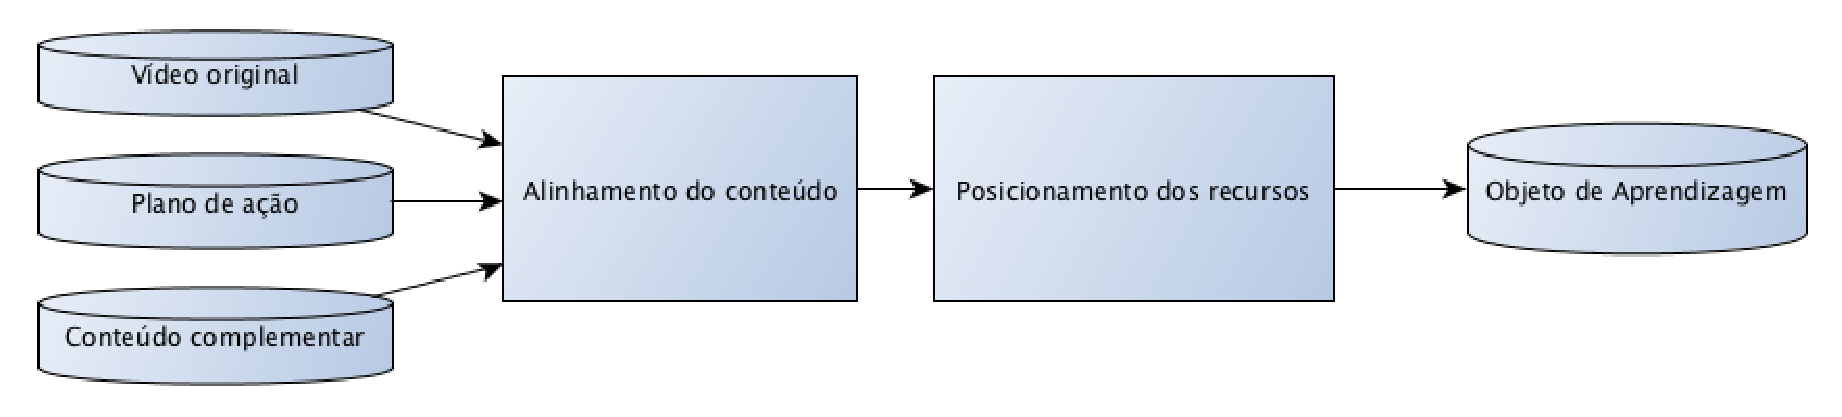
\includegraphics[width=.99\textwidth]{imagens/metodo/fase4_oa.eps}
\caption{Fase 4 do método}
\label{fig:metodo:fase4}
\end{figure}

Finalmente, cada artefato que compõe o conteúdo complementar é posicionado em relação ao vídeo de acordo com as definições do plano de ação, e desta forma o objeto de aprendizagem é finalizado.

